\documentclass[letterpaper,12pt]{article}
\usepackage{tabularx} % extra features for tabular environment
\usepackage{amsmath}  % improve math presentation
\usepackage{float}
\usepackage{pdfpages}


\usepackage{graphicx} % takes care of graphic including machinery
\graphicspath{ {./figures/} }
%\usepackage[margin=1in,letterpaper]{geometry} % decreases margins
%\usepackage{cite} % takes care of citations
\usepackage[final]{hyperref} % adds hyper links inside the generated pdf file
\hypersetup{
	colorlinks=true,       % false: boxed links; true: colored links
	linkcolor=blue,        % color of internal links
	citecolor=blue,        % color of links to bibliography
	filecolor=magenta,     % color of file links
	urlcolor =blue         
}
\usepackage[margin = 1in,headsep=0.5cm,headheight=2cm,letterpaper]{geometry} 

\usepackage{fancyhdr}
\pagestyle{fancy}
\lhead{Student 1 : Ahmet Akman 2442366 \\ Student 2: Yusuf Toprak Yıldıran 2444149 \\ Assistant: Onur Selim Kılıç}
\rhead{Date: \today \\ Group: Wednesday Morning - 5} 
%\cfoot{center of the footer!}
\renewcommand{\headrulewidth}{0.1pt}



\begin{document}
\thispagestyle{empty}

\title{Spring 2022 EE214 Experiment 3  \protect\\ Transformers and MATLAB Workshop }
\author{Ahmet Akman 2442366 \protect\\ Yusuf Toprak Yıldıran 2444149 \protect\\ Assistant: Onur Selim Kılıç}
\date{\today}
\maketitle
\tableofcontents
%\begin{abstract}
%abstract
%\end{abstract}
\section{Introduction}
In this experiment, transformers and MATLAB workshop, we are required to get used to plotting with MATLAB and experimented with different transformer setups. First, we are expected to observe the step-down property of the transformer. Then, the behavior of the transformer with a resistive load is expected to have experimented with different frequencies. The transformer's characteristics are needed to be formulated with an equivalent circuit. Lastly, the advantage of the impedance matching circuit setup is requested to be observed.
\section{Experimental Results and Discussion}
The results of the experiment are discussed in the following steps.
%
\subsection{Step 1}

In this step transformer circuit with no resistive load is examined.
\begin{figure}[H]
    \centering
    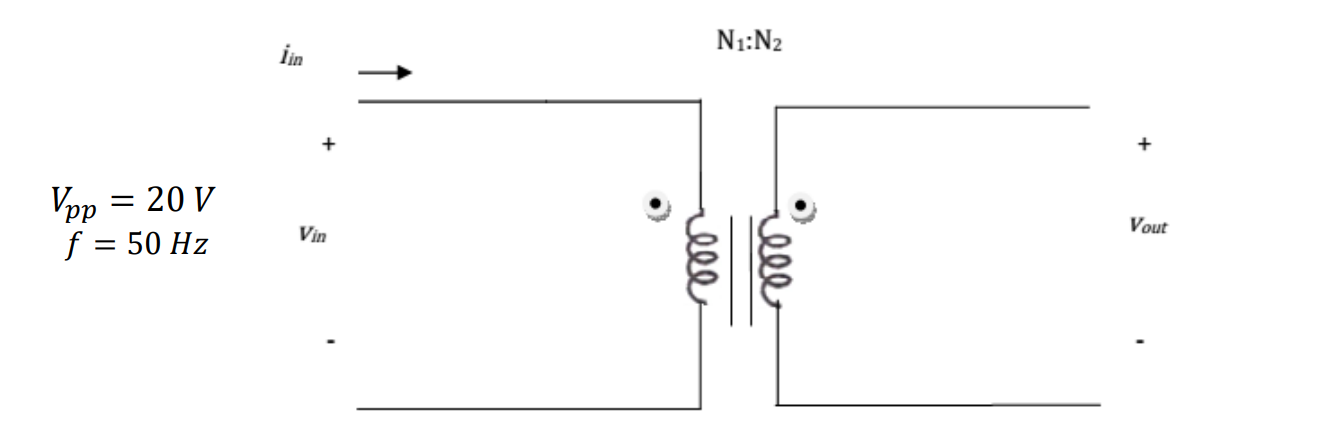
\includegraphics[width = 0.75\textwidth]{1.png}
    \caption{Circuit schematic for the step 1}
\end{figure} 


In the first step, the following circuit given in Figure 1 is set, and it is observed that the step-down operation of the transformer under no load with sinusoidal input voltage has a peak to peak voltage of 20 V and frequency of 50 Hz. Then, \(V_{in}(t) \) and \(V_{out}(t)\) are plotted on the graph in Figure 2.
\begin{figure}[H]
    \centering
    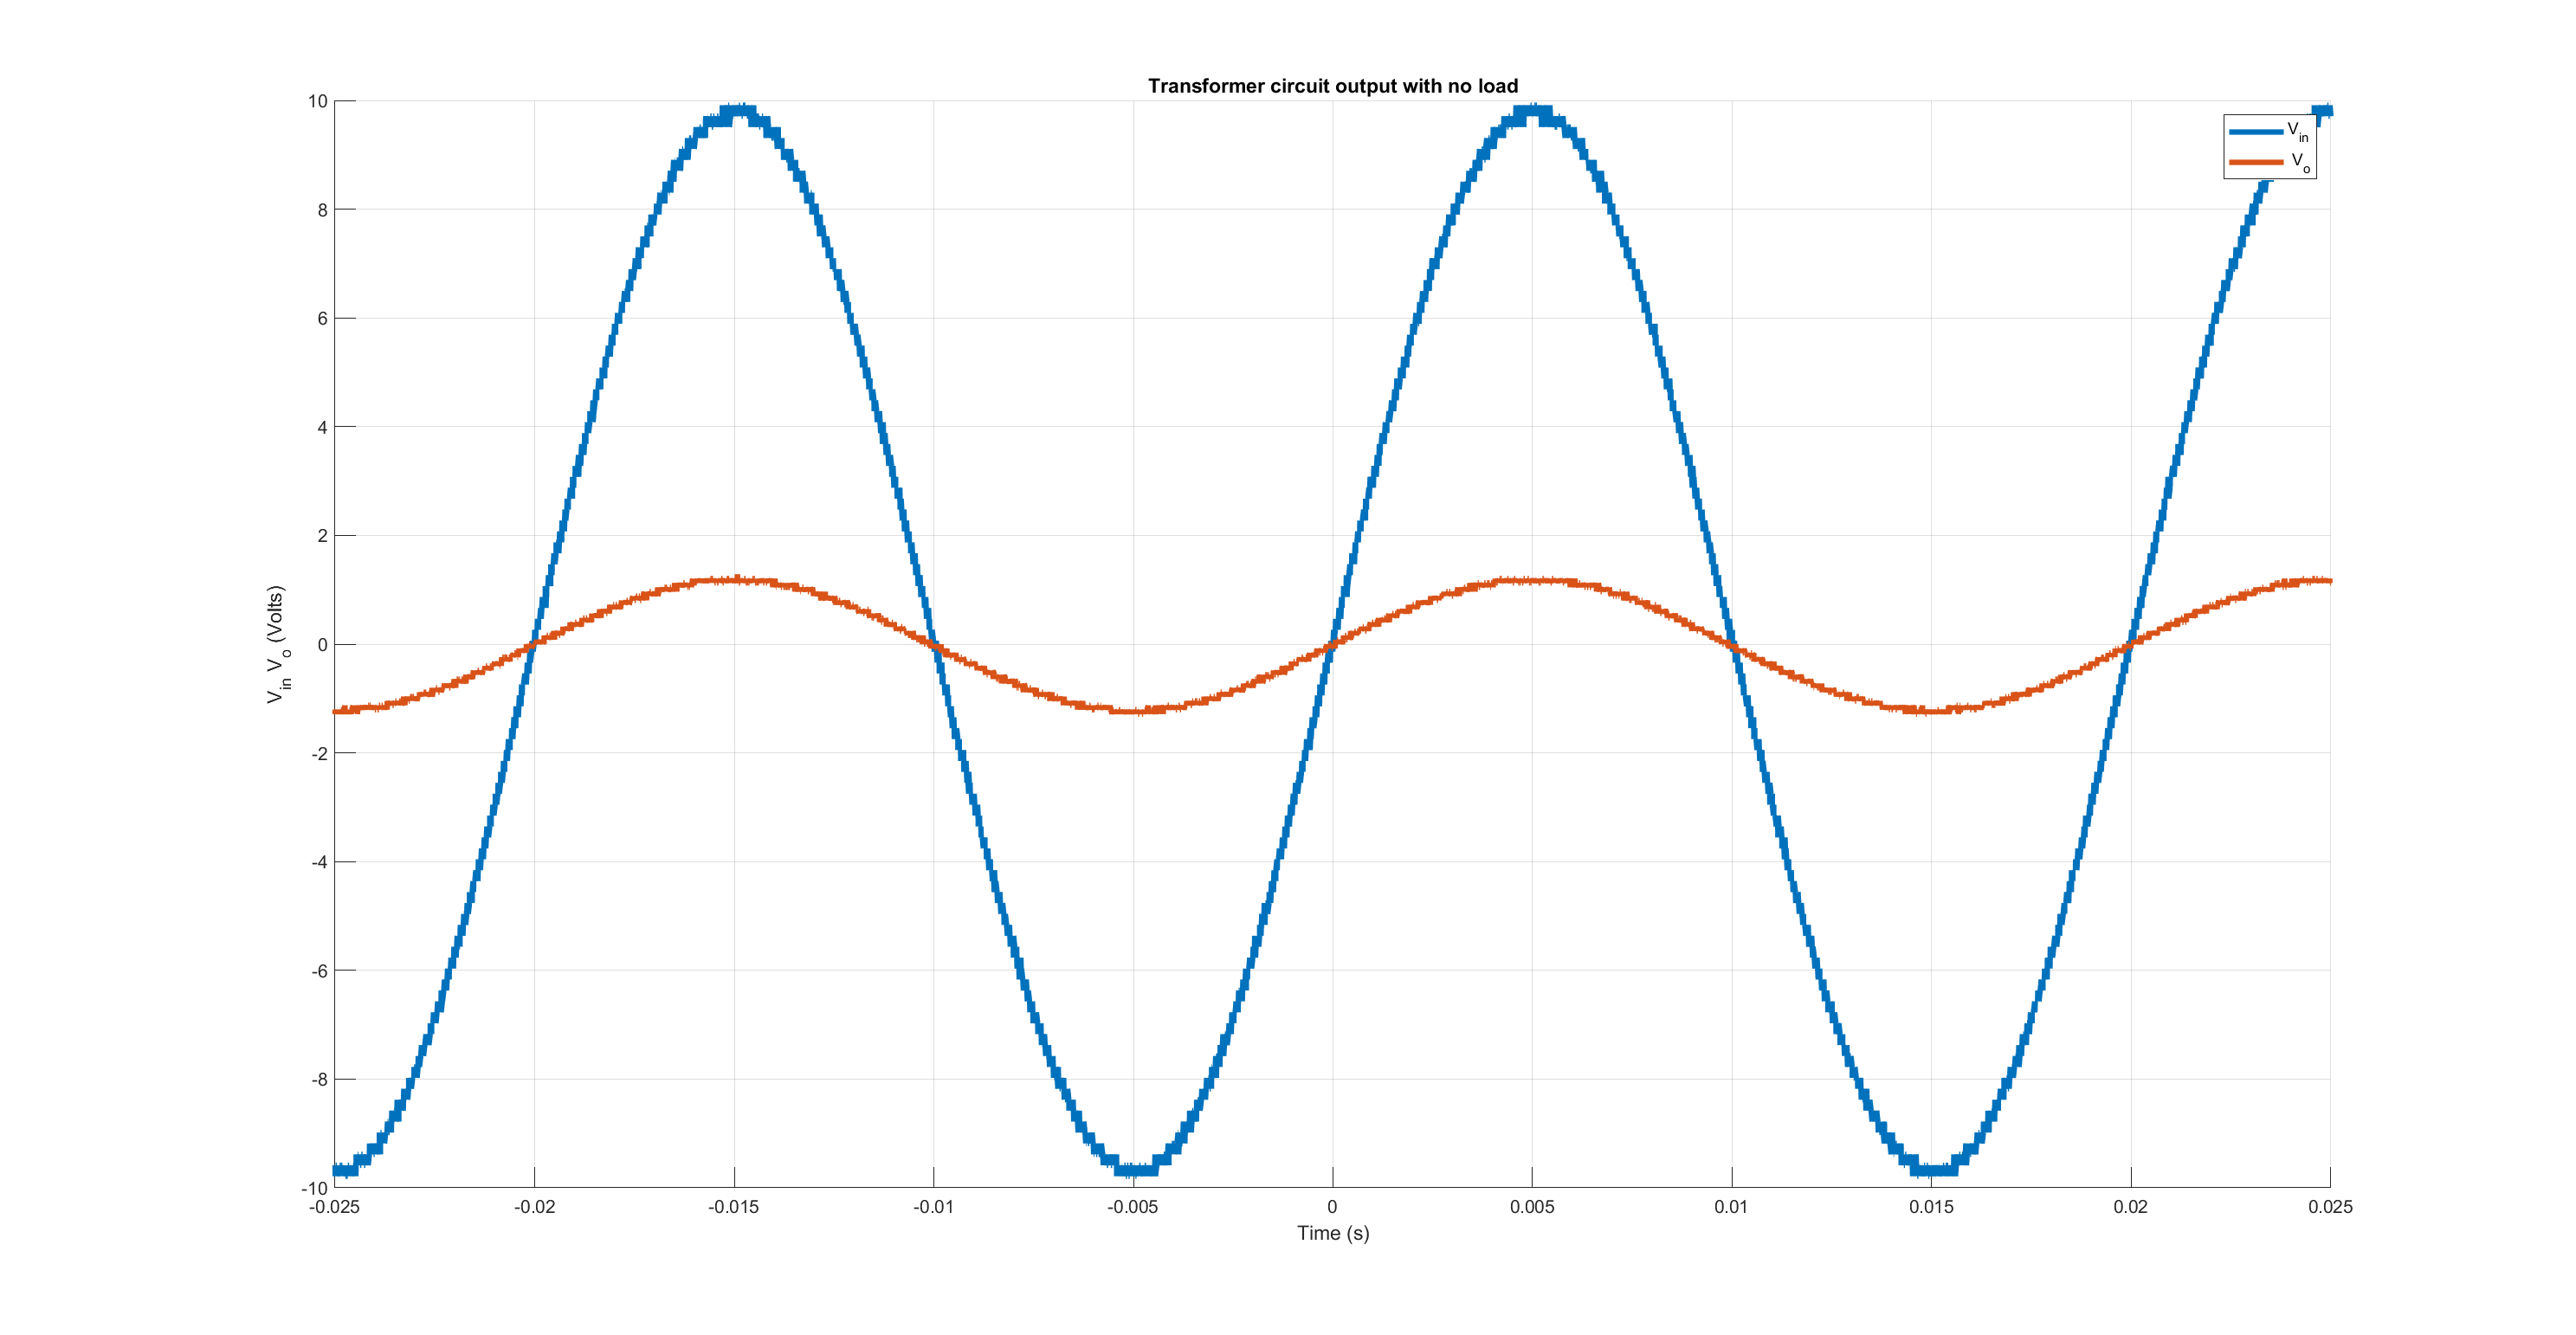
\includegraphics[width = 1\textwidth]{1_1.png}
    \caption{\(V_in(t) \) and \(V_out(t)\) vs Time}
\end{figure} 
Afterwards, \(N_1:N_2\) ratio is measured as \(\frac{19.5}{2.5}\approx 7.8 \).

%

%
\subsection{Step 2}
In this step transformer circuit with a resistive load is examined.
\begin{figure}[H]
    \centering
    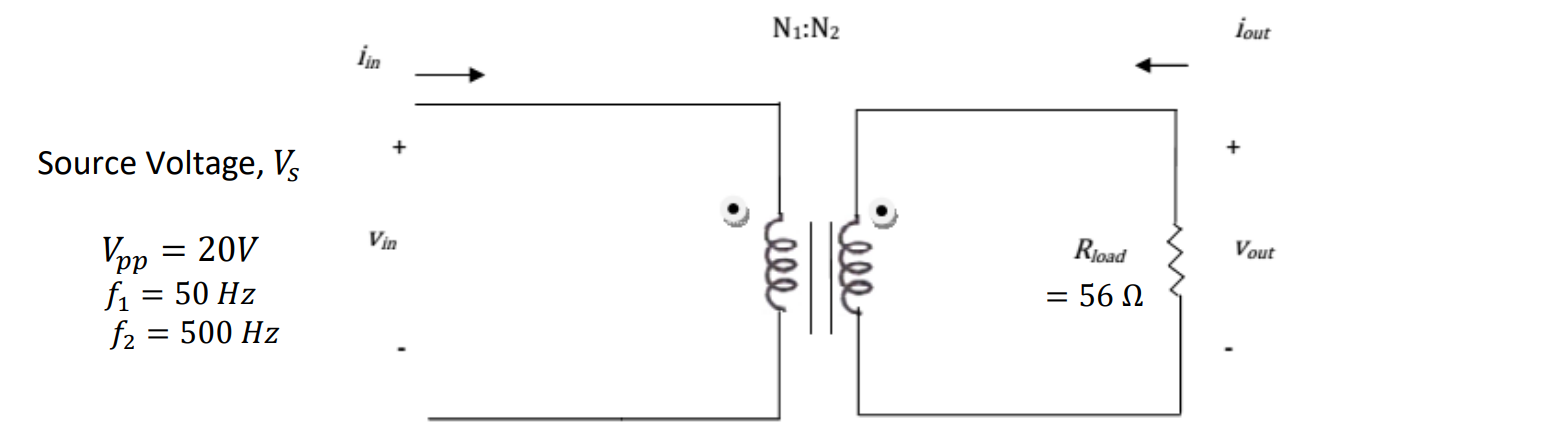
\includegraphics[width = 0.75\textwidth]{2.png}
    \caption{Circuit schematic for the step 2}
\end{figure} 


For this step, the signal generator output is adjusted as \(V_s = 10sin(2\pi50t)\) with 20V peak to peak voltage and 50Hz frequency; then, the Transformer circuit with resistive load is constructed as given in Figure 3, where R = \(56\Omega \).  
\subsubsection{i}
In this step, to obtain current \(I_{in}\), \(1K\Omega \) resistor is connected between the - terminal of the primary side transformer and the - terminal of the signal generator. Then, CH1 is connected to the + terminal of the signal generator, and the CH2 probe is to the - terminal of the primary side transformer. By subtracting CH2 from CH1 \(V_{in}\) is obtained, and the CH2 probe of DSO gives \(I_{in}\) in mA. Afterwards, \(V_{in}\) and \(I_{in}\) are plotted in Figure 4. 

\begin{figure}[H]
    \centering
    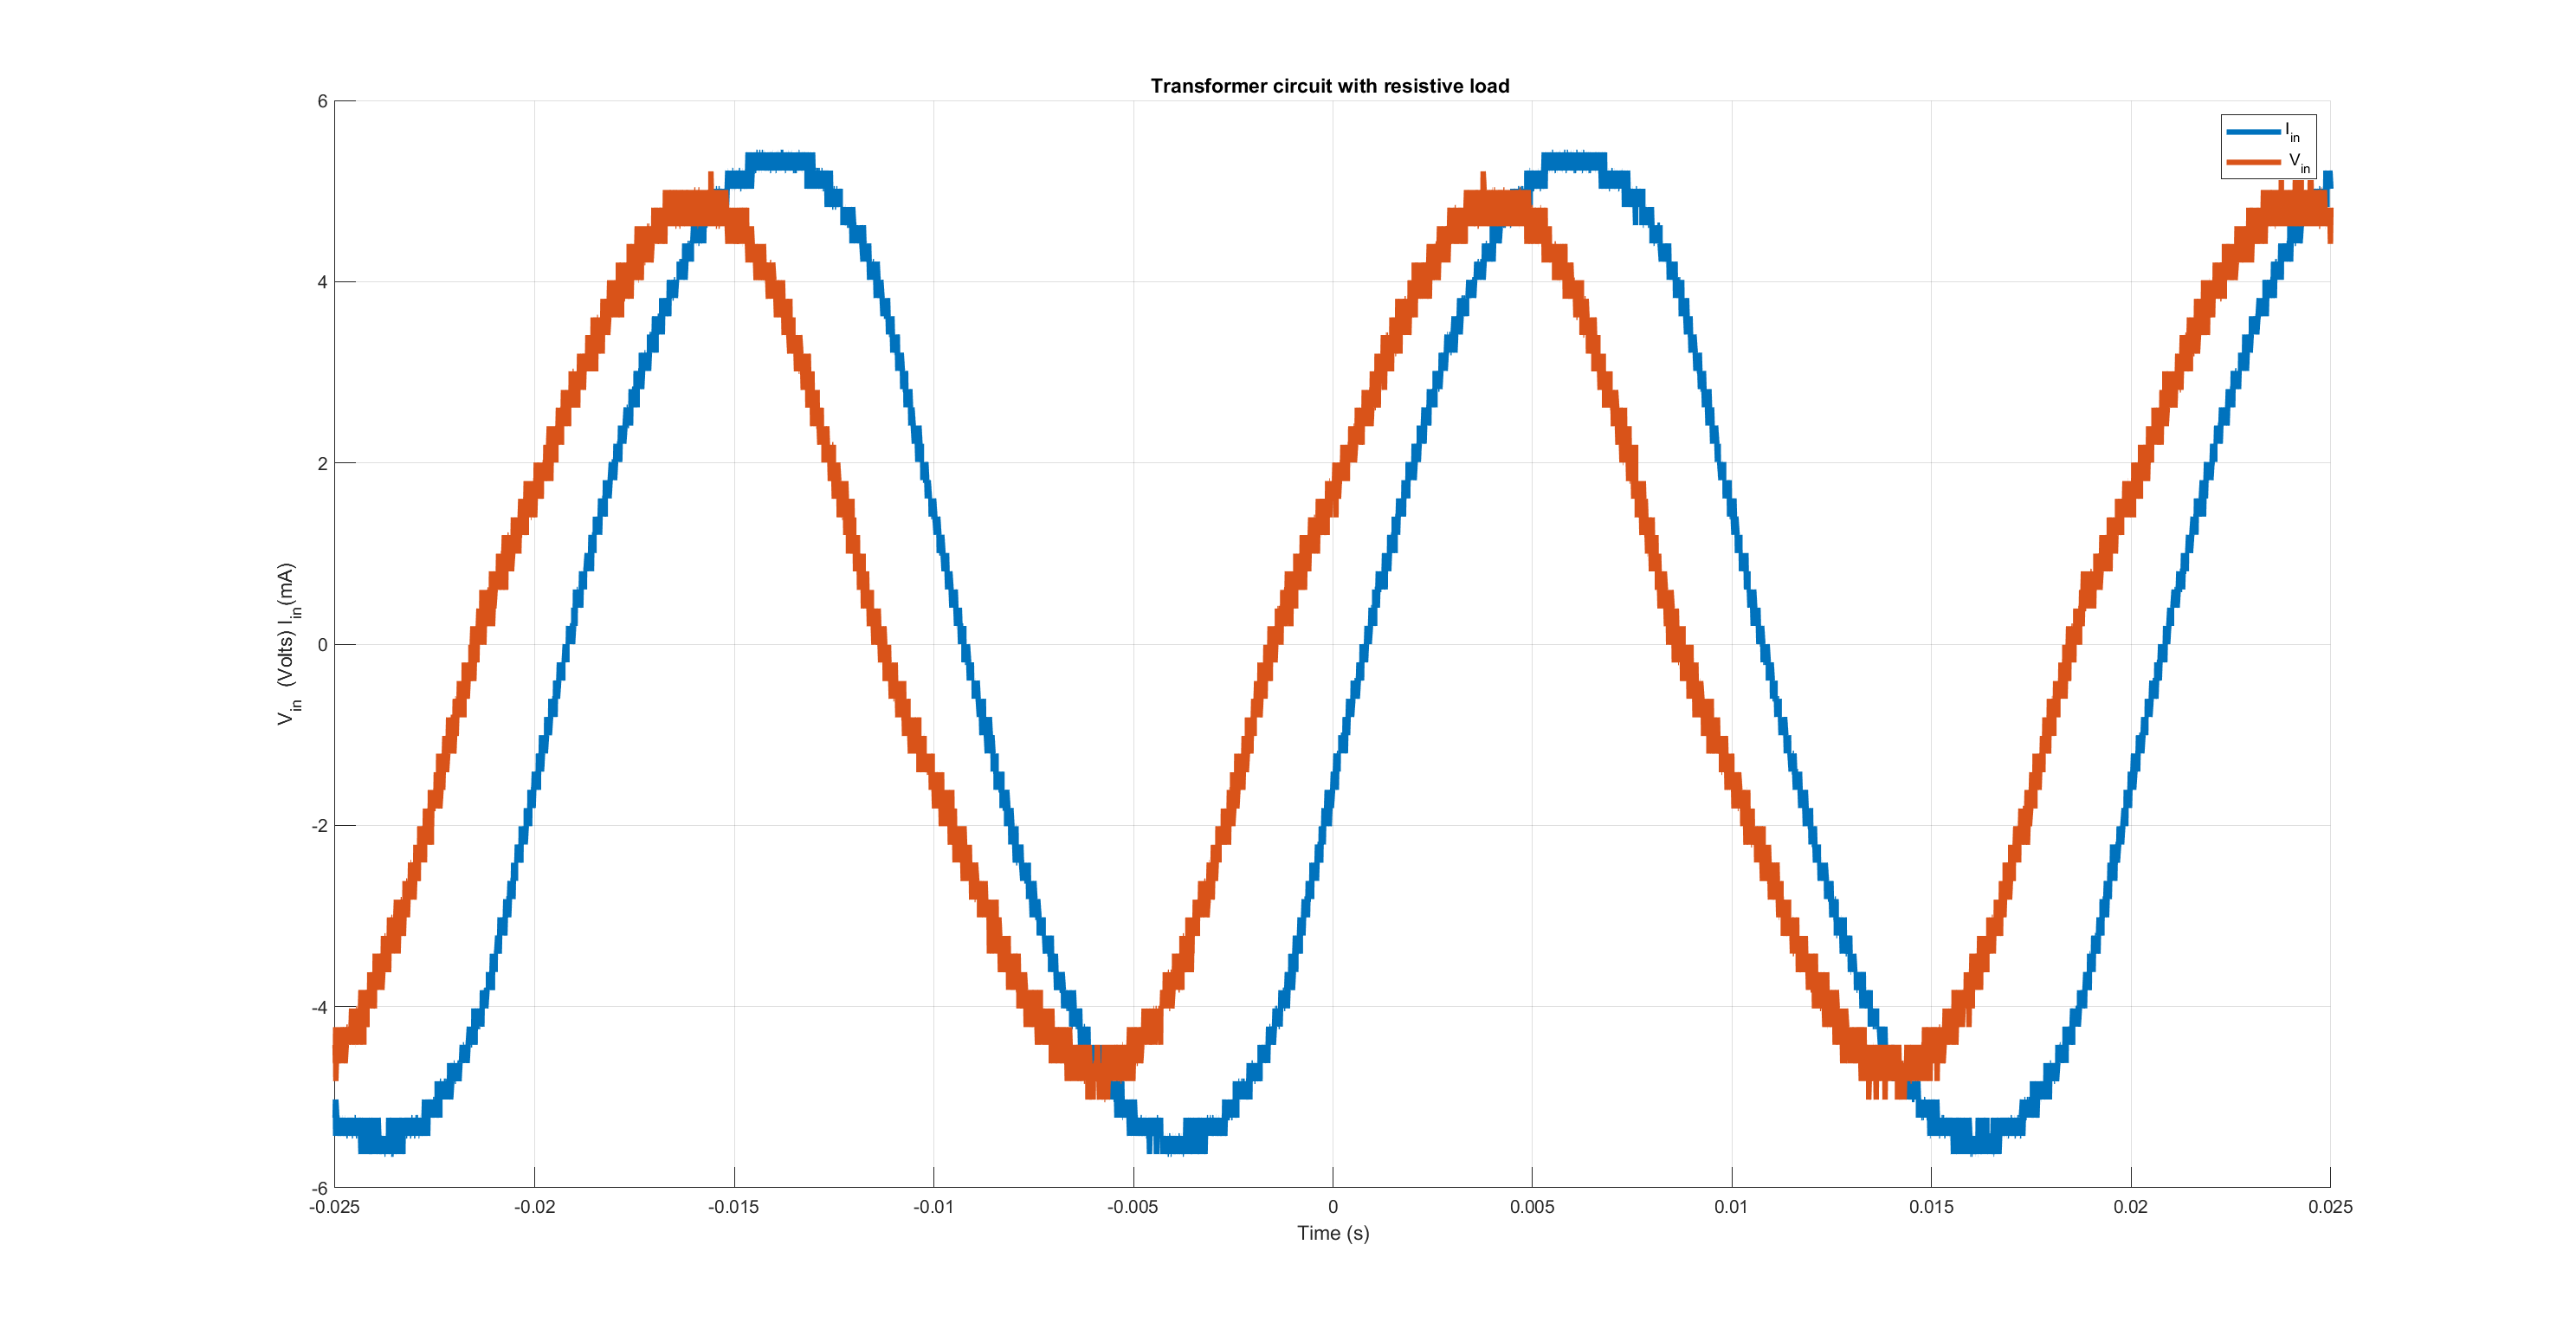
\includegraphics[width = 1\textwidth]{2_1.png}
    \caption{\(V_in(t) \) and \(I_in(t)\) vs Time}
\end{figure} 
Then, \(V_{rms}\), \(I_{rms}\) and \(P_{in}\)(\(P_{in}\) = \(V_{rms} \times\)\(I_{rms}\) )  are obtained using the DSO measurement tool as 3.5V and 3.7mA, respectively, given in Table 1.
\begin{table}[H]
    \begin{center}
        \caption{RMS Values of input \(V_{rms}\) and input \(I_{rms}\) and \(P_{in}\)}
        \vspace{2mm}
        \begin{tabular}{||c | c | c ||} 
            \hline
            \(V_{rms}\) & \(I_{rms}\) & \(P_{in}\) \\ [0.5ex] 
            \hline\hline
            3.5 V & 3.7 mA & 12.95mW   \\
            \hline
        \end{tabular}
    \end{center}
\end{table}

\subsubsection{ii}
For this step, CH1 is connected to the + terminal of the secondary side of the transformer, and from that, probe \(V_{out}(t)\) is obtained and plotted as in Figure 5. Then, the RMS value of \(V_{out}\) is measured with DSO as 555mV. Then, \(P_{out}\) is calculated as \(\frac{V_{out}^2}{56\Omega } = 5.5mW\). The reason for \(P_{out}\) is less than \(P_{in}\) is because the circuit is not ideal.
\begin{figure}[H]
    \centering
    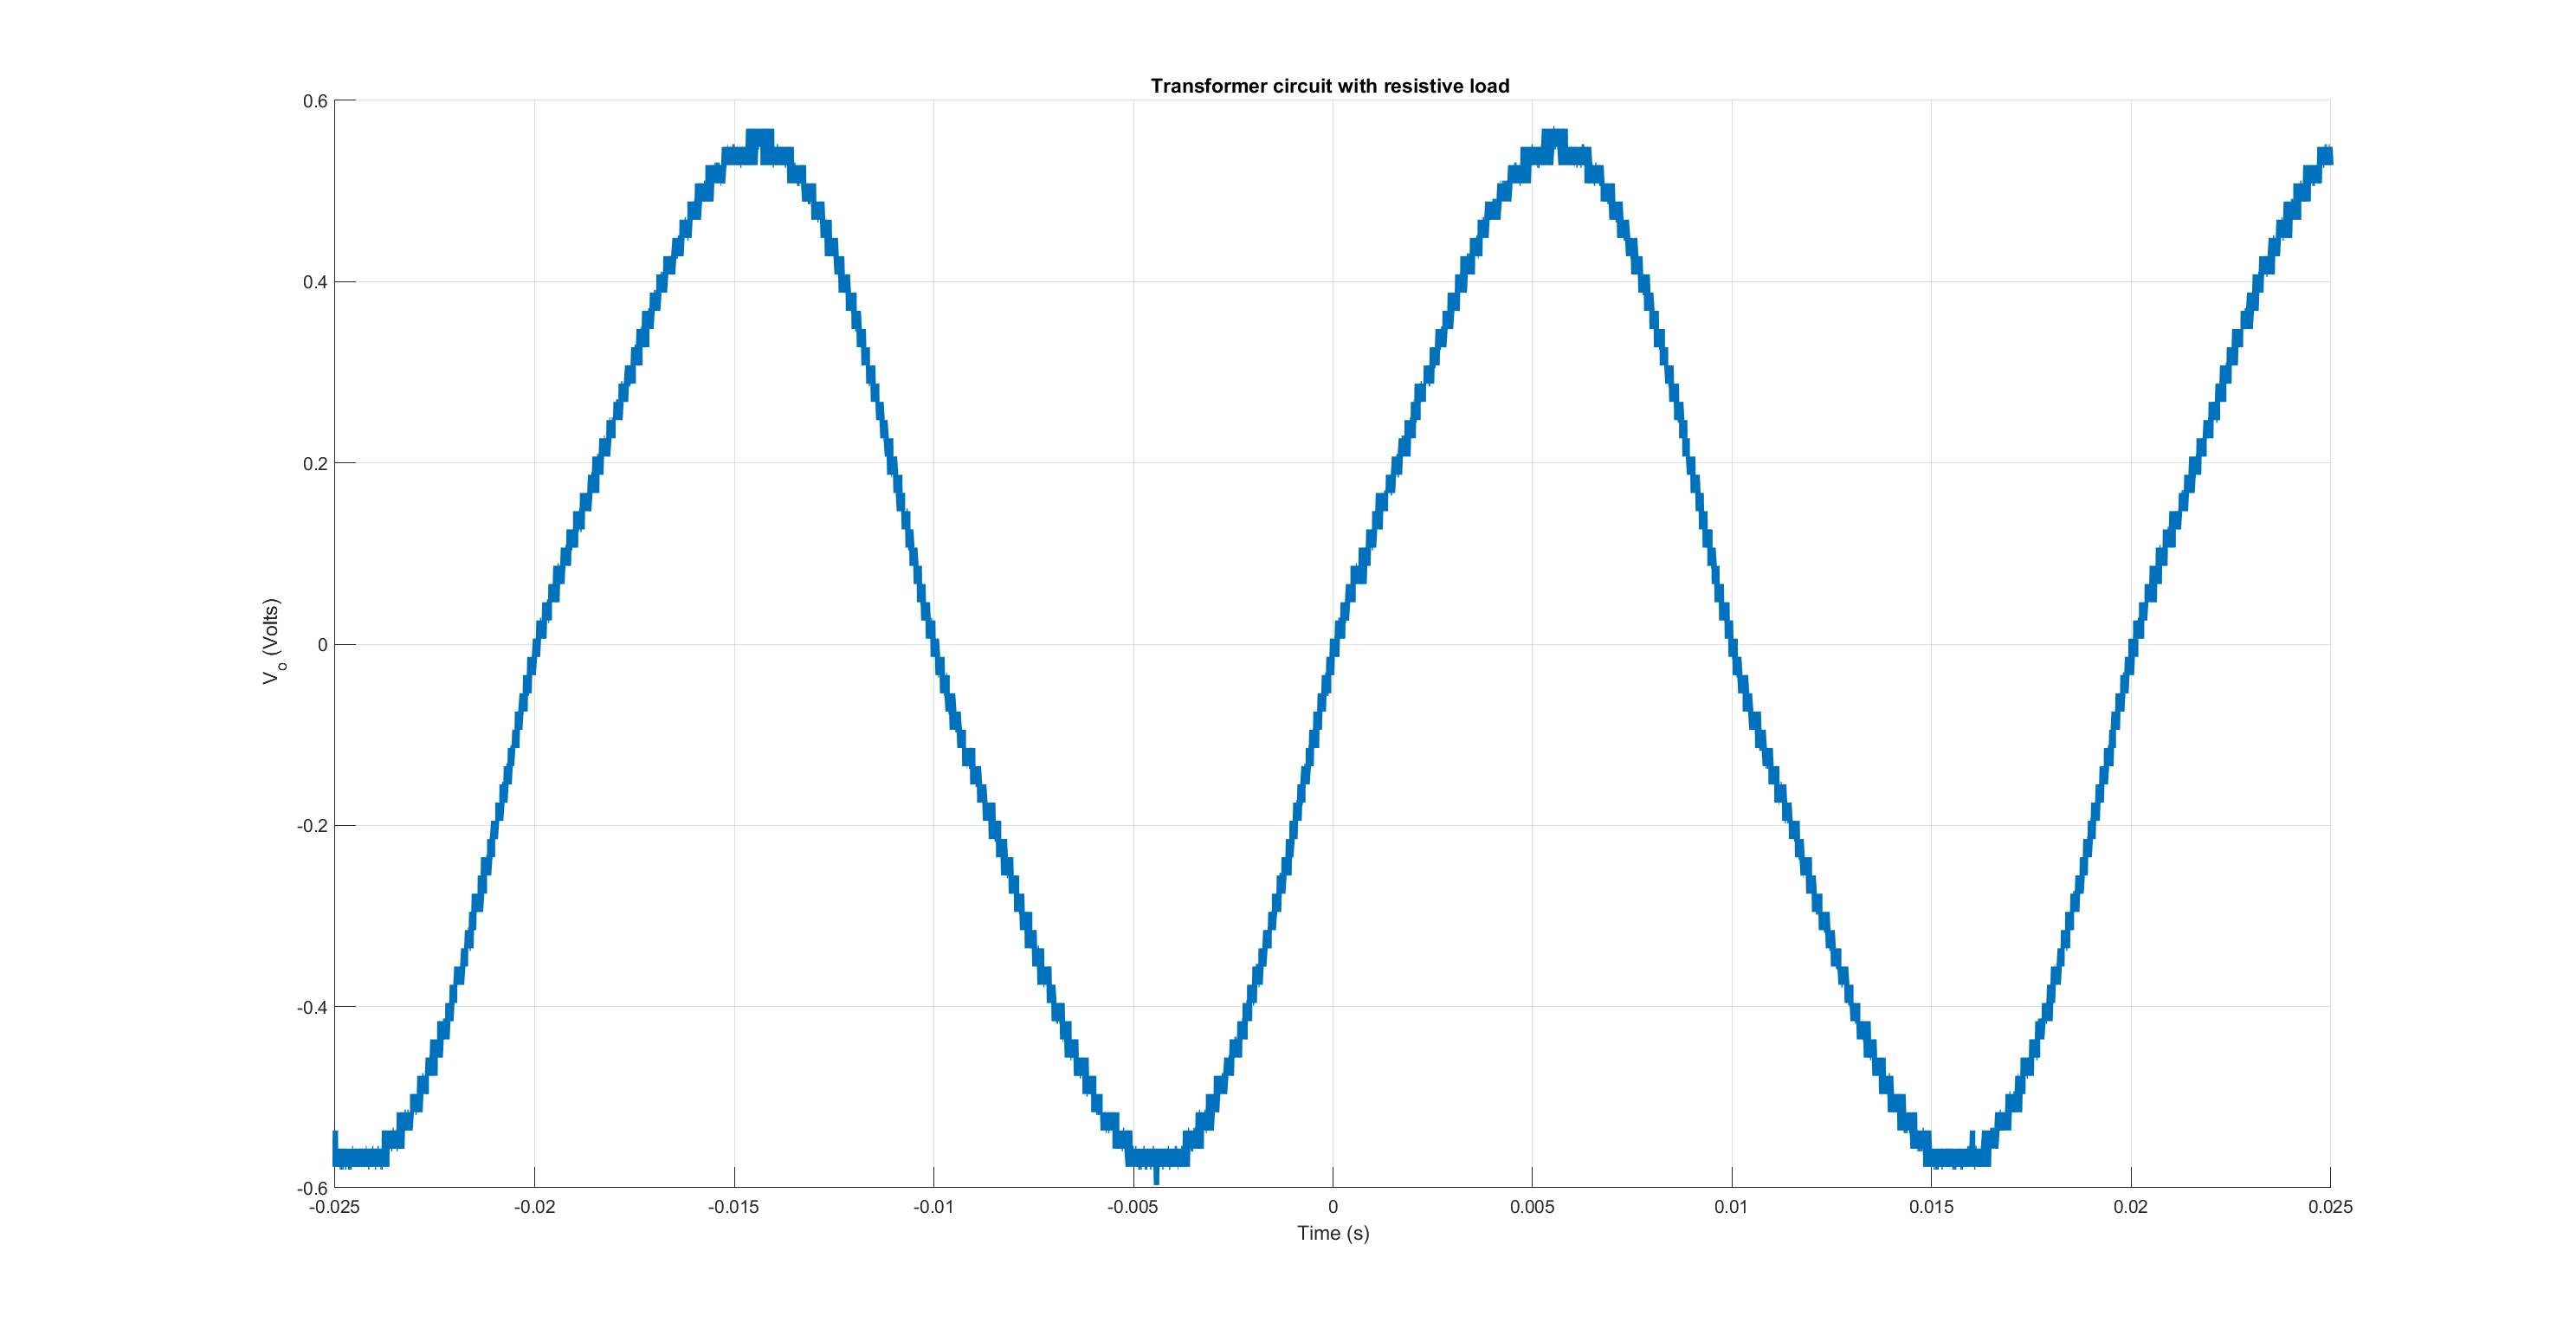
\includegraphics[width = 1\textwidth]{2_2.png}
    \caption{\(V_o(t) \) vs Time}
\end{figure} 

\subsubsection{iii}
In this step, input frequency is increased to 500 Hz, and i. and ii. are repeated. The plots given in Figures 6 and 7 are obtained.
\begin{figure}[H]
    \centering
    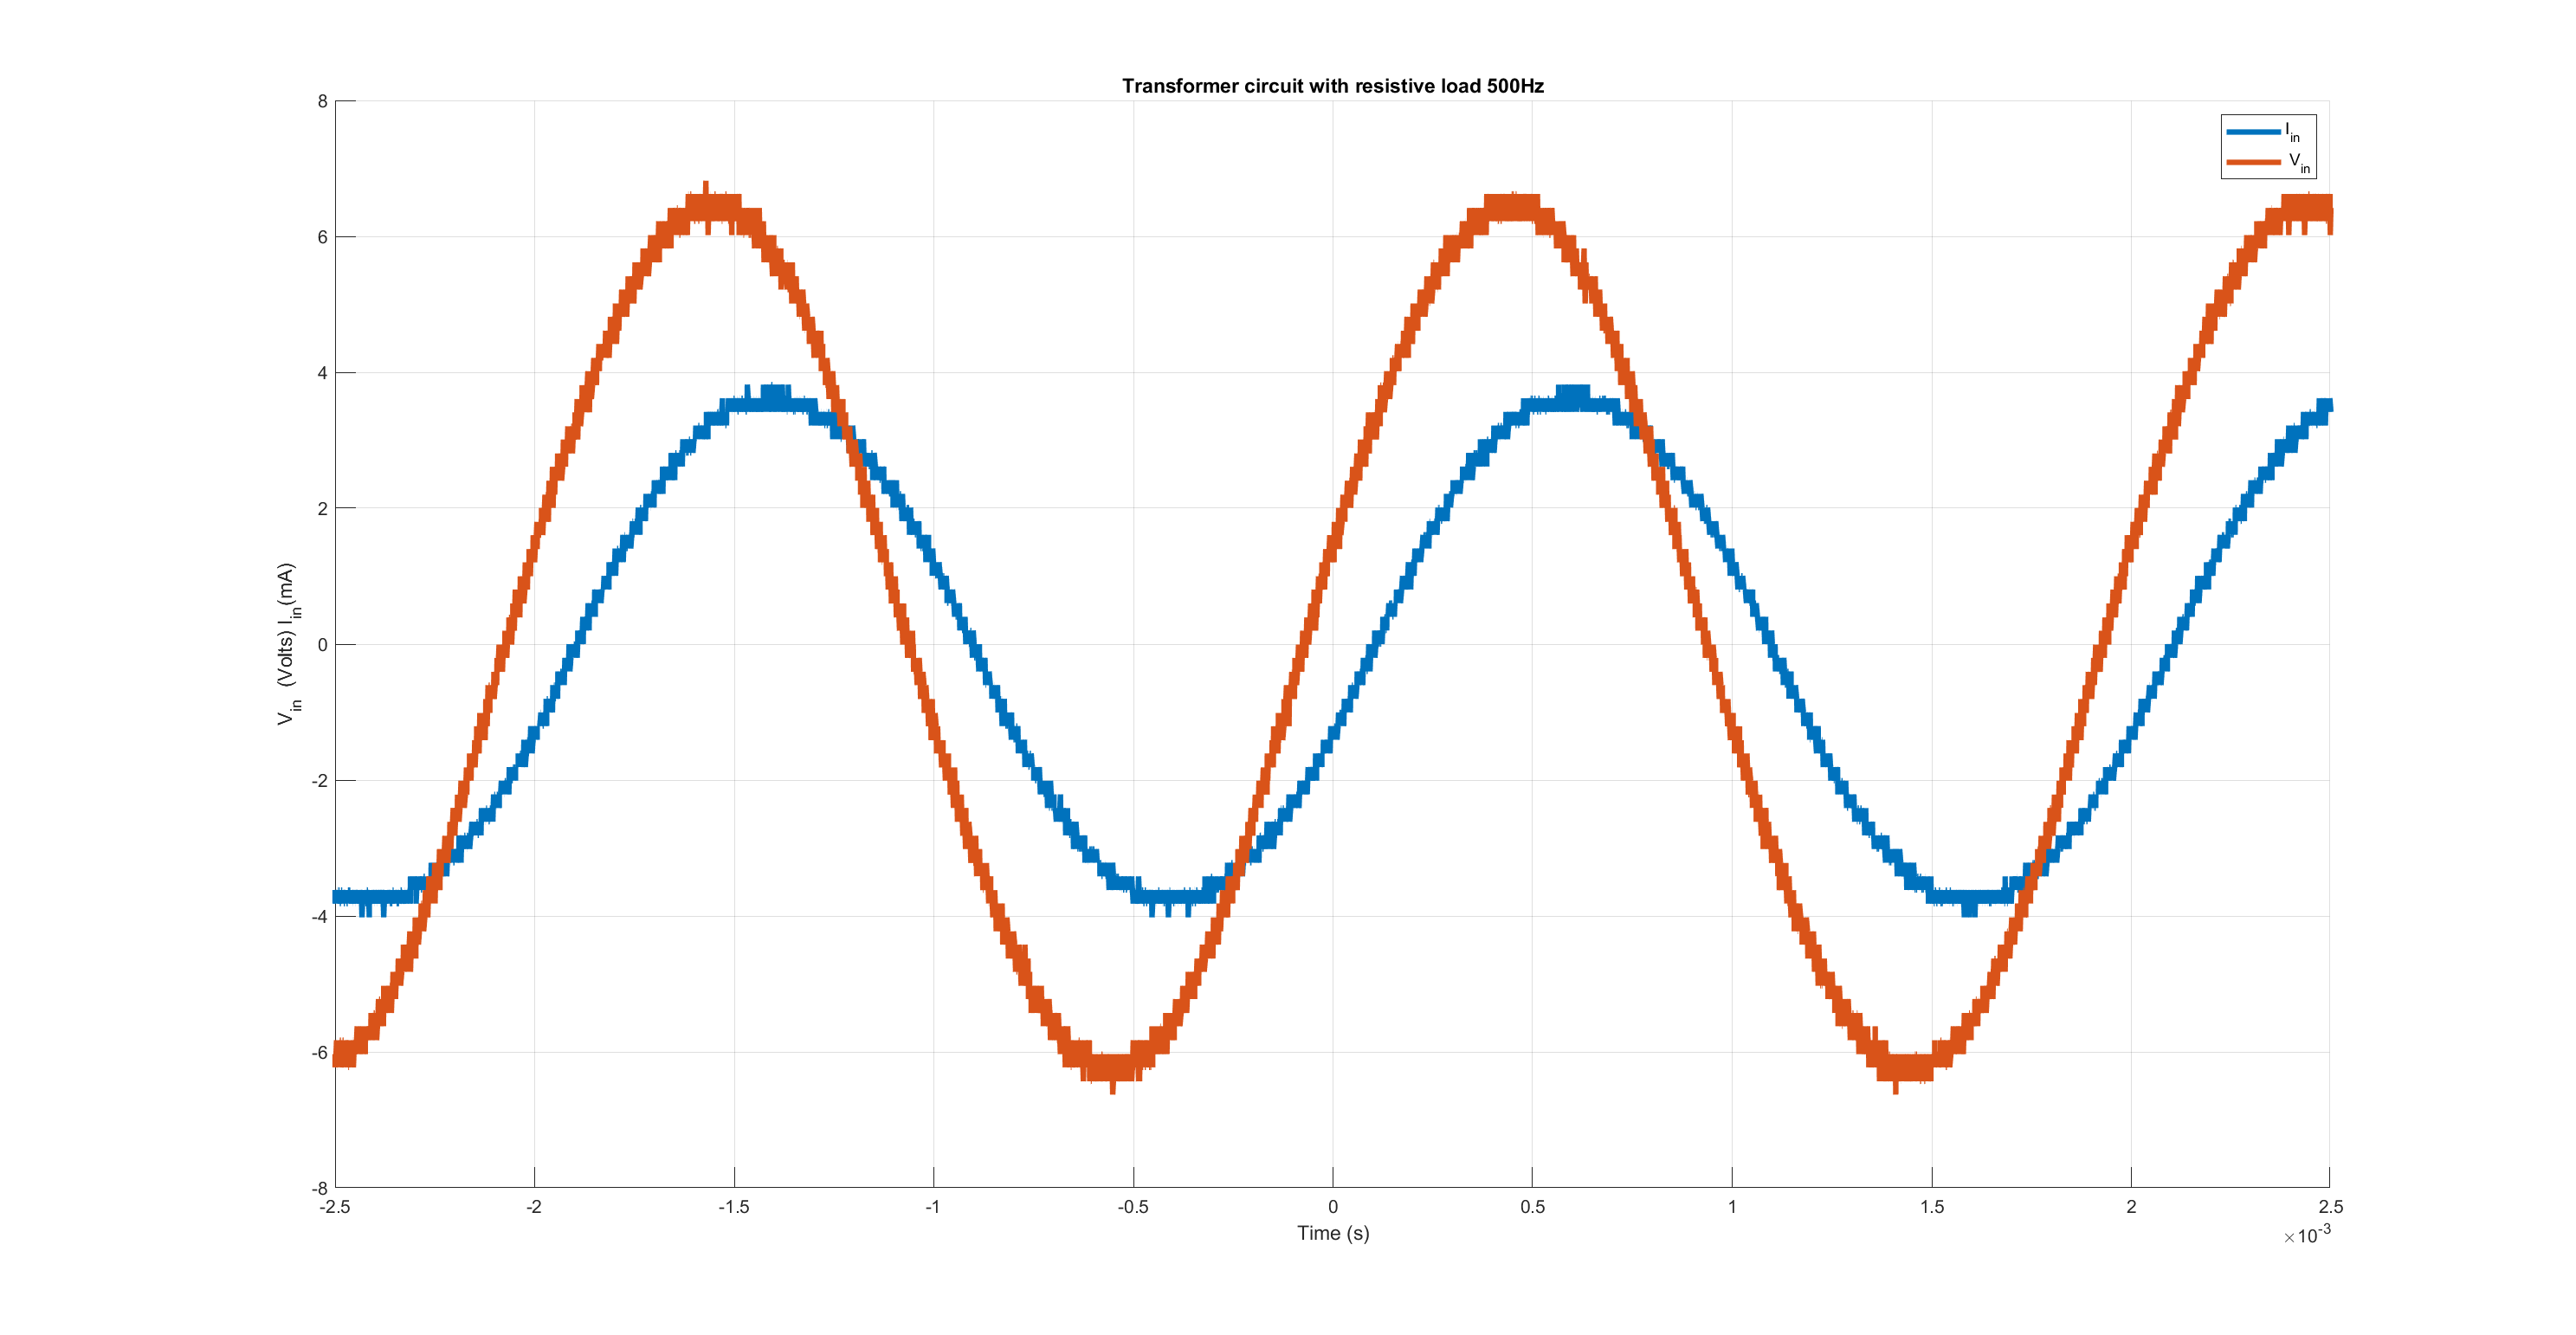
\includegraphics[width = 1\textwidth]{2_3_1.png}
    \caption{\(V_{in}(t) \) and \(I_{in}(t)\) vs Time (500Hz)}
\end{figure} 

\begin{figure}[H]
    \centering
    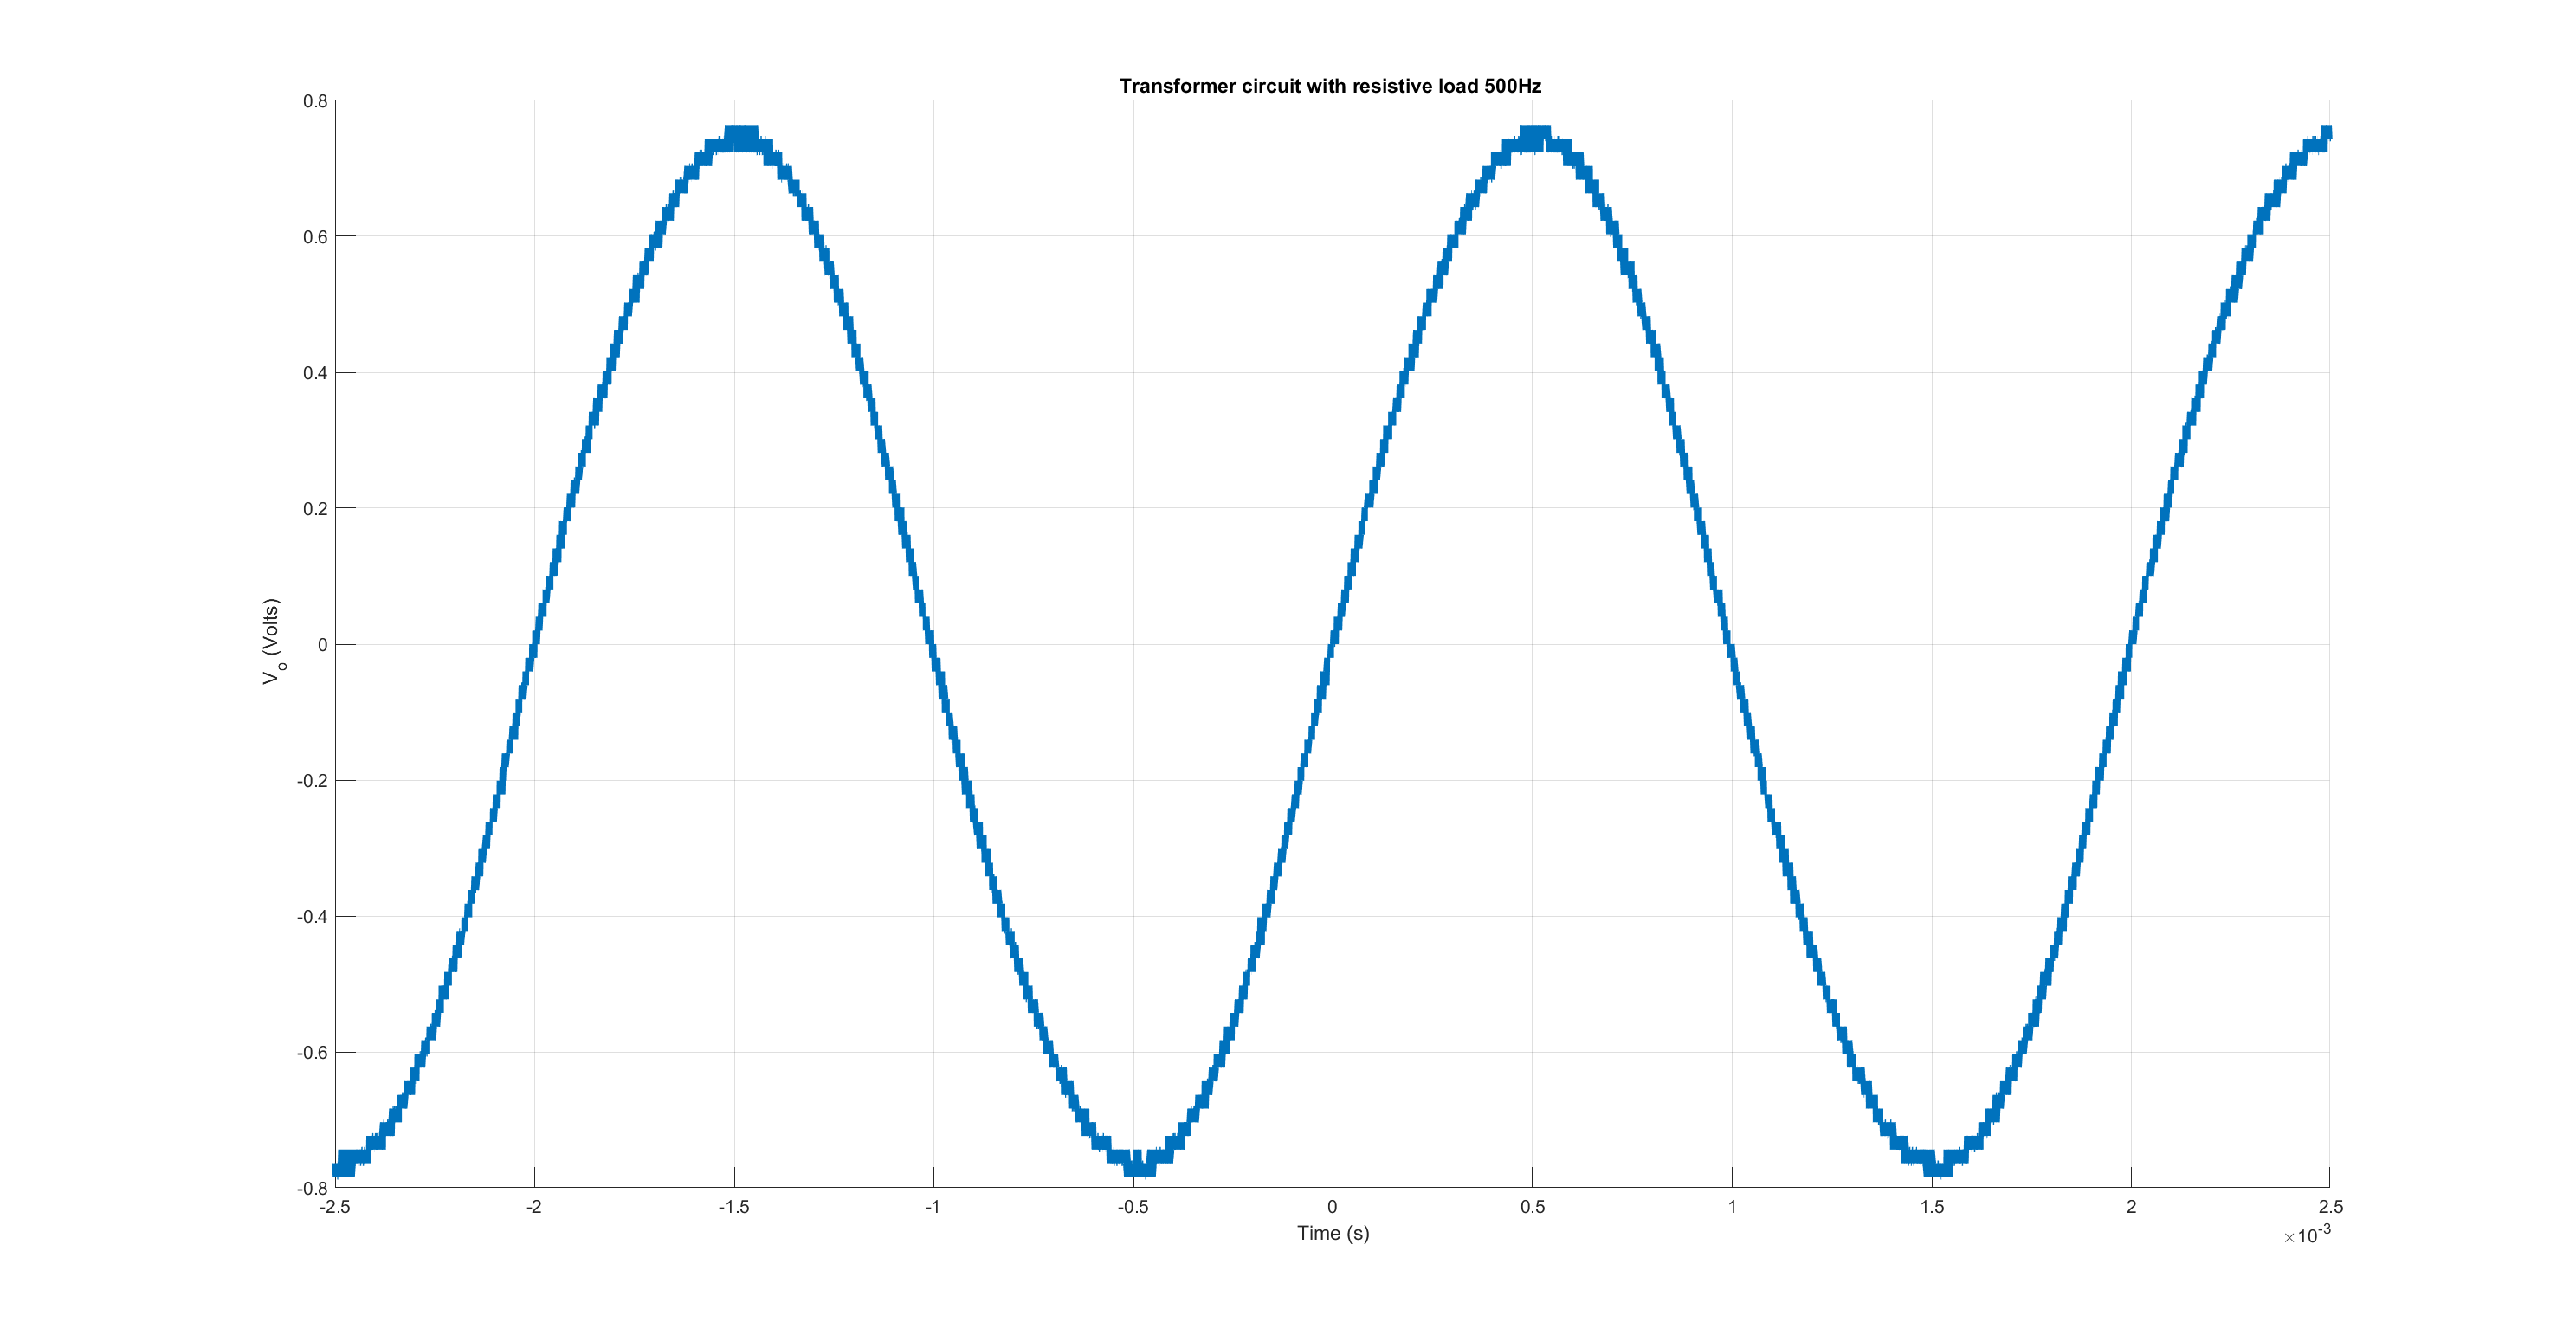
\includegraphics[width = 1\textwidth]{2_3_2.png}
    \caption{\(V_o(t) \) vs Time (500Hz)}
\end{figure} 

In previous steps (i. and ii.), the phase difference between voltage and the current was measured as \(-40\deg \), and when the frequency is increased to 500 Hz phase difference is obtained as \(-25\deg\). Therefore, it is clearly seen that as frequency increases phase difference between voltage and current decreases. But after some point, although the frequency continues to increase, the rate of change in phase difference decreases less and less. 
%
\subsection{Step 3}
In this step transformer equivalent circuit is formulated by making the secondary terminal of the transformer short-circuited.
\subsubsection{i}


%
By connecting a 1K\(\Omega\) resistor series to the primary terminal, we have obtained the plot given in Figure 8, which shows \(V_{in}(t) \) and \(I_{in}(t)\) on the same graph.  
\begin{figure}[H]
    \centering
    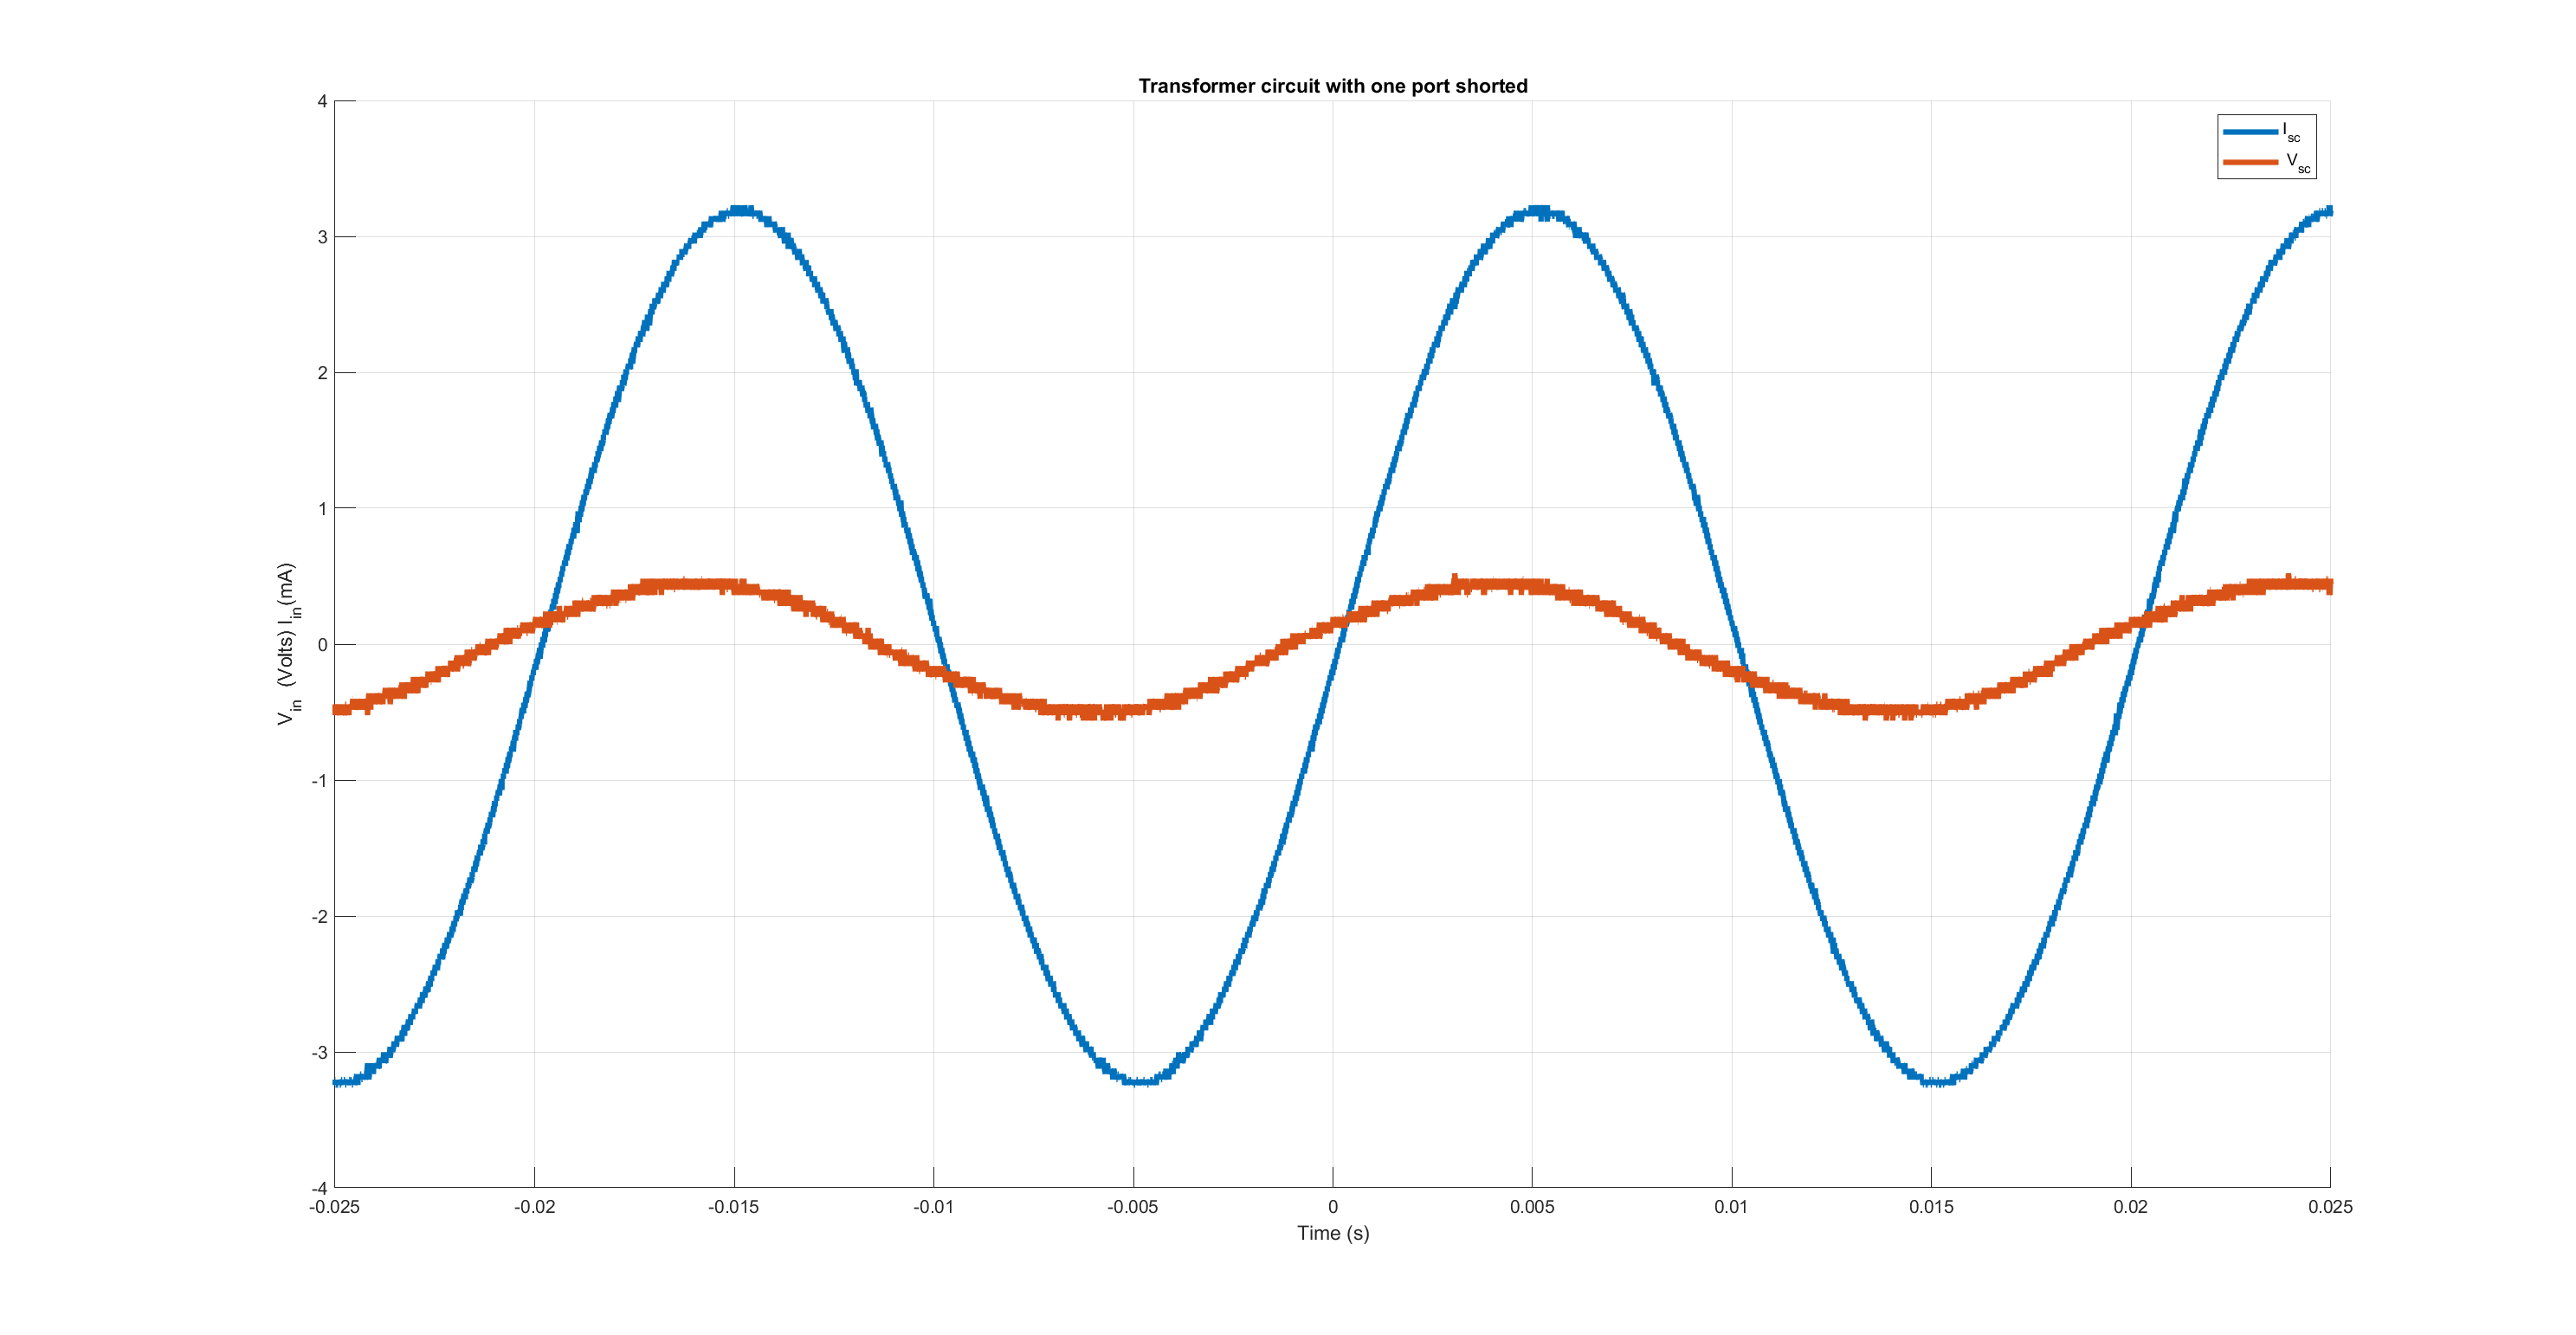
\includegraphics[width = 1\textwidth]{3_1.png}
    \caption{\(V_{in}(t) \) and \(I_{in}(t)\) vs Time }
\end{figure} 

\subsubsection{ii}
A bunch of assumptions and calculations is made to obtain the equivalent circuit parameters given in Figure 9.
\begin{figure}[H]
    \centering
    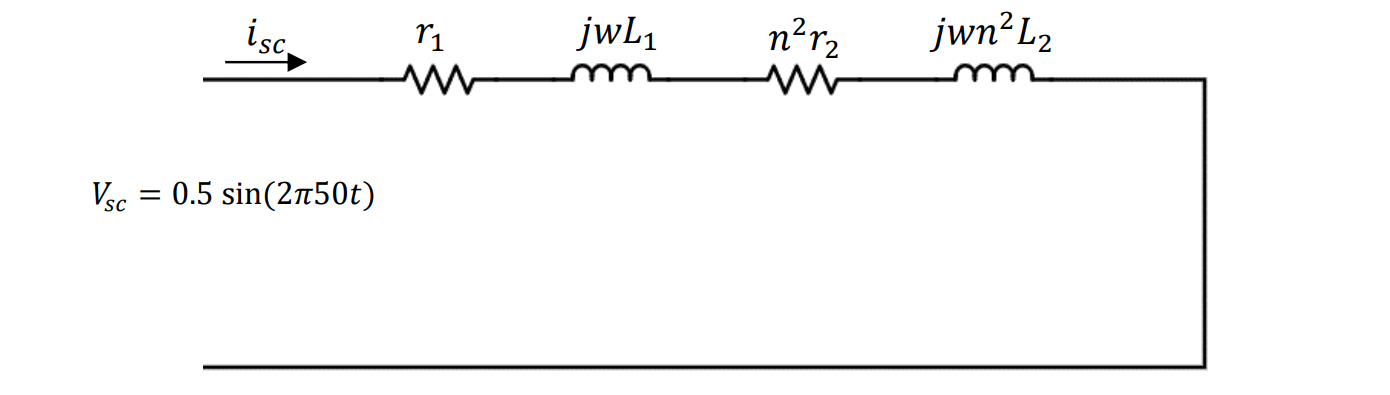
\includegraphics[width = 0.75\textwidth]{3.png}
    \caption{Transformer equivalent circuit}
\end{figure} 
From the measurement feature of the oscilloscope, \(V_{sc-RMS}\) and \(I_{sc-RMS}\) are found to be 0.3345 Volts and 0.0230 Amps, respectively. So the impedance becomes;
\[
    Z = \frac{V_{sc-RMS}}{I_{sc-RMS}} = 150 \Omega
    \]
    The primary side of the resistance and inductance is taken equal to the reflected equivalent secondary side of resistance and inductance. The \(\theta\), phase difference is found as 23.9326 degrees. The resistance becomes;
    \[
    R = Z cos (\theta) = 137.103
    \]
    The reactance becomes;
    \[
    X = Z sin (\theta) = 60.849 
    \]
    So, as a result, the parameters given in Table 2 are obtained by equating the overall resistance to R and overall reactance to X. From Step 1, n is taken as 8.
    \begin{table}[H]
    \begin{center}
        \caption{Transformer equivalent circuit parameters}
        \vspace{2mm}
        \begin{tabular}{||c | c | c | c ||} 
            \hline
            \(r_1 (\Omega) \) & \(r_2 (\Omega)\)  & \(L_1\) (H) & \(L_2\) (H) \\ [0.5ex] 
            \hline\hline
            68.553 & 1.071 & 0.30425 & 0.00475 \\ 
            \hline
        \end{tabular}
    \end{center}
    \end{table}
    

    %
\subsection{Step 4}
In this step impedance matching transformer circuit is constructed as it is in Figure 10 with the input \(V_{in}(t) = 10sin(2\pi50t)\) and same \(N_1:N_2\) rate. 
\begin{figure}[H]
    \centering
    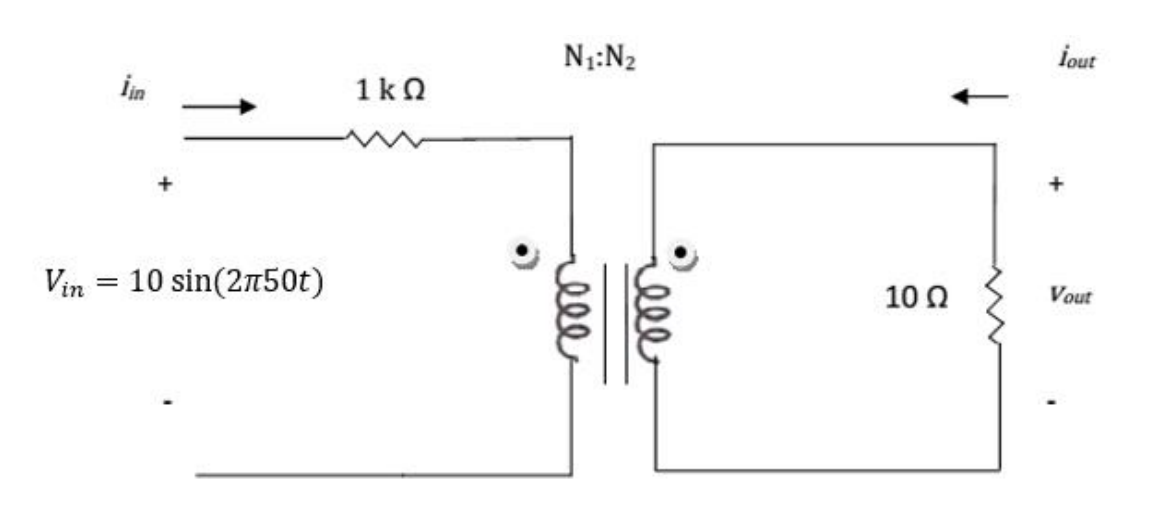
\includegraphics[width = 0.75\textwidth]{4.png}
    \caption{Impedance matching}
\end{figure} 

\subsubsection{i}
For this step, an impedance matching transformer circuit is used. In order to obtain \(V_{out}\) CH1 is connected + terminal of the secondary side of the transformer, and power dissipated is calculated as follows:
\[\frac{V^2}{R} = \frac{(V_{rms})^2}{R} = \frac{0.216^2}{10\Omega } = 0.0046 Watt\]   

\subsubsection{ii}
For this step, 1K\(\Omega \) and 10\(\Omega \) resistors are connected series without the transformer and the same calculation is made in i. :
\[\frac{V^2}{R} = 4.9 \times 10^{-4} Watt\]
From these results, it is seen that in the second case, power transmitted to 10\(\Omega \) from the same input is significantly smaller than in the first. Therefore, we can conclude that transformers can be used for delivering power efficiently. 

\section{Conclusion}
In this experiment, transformers and MATLAB workshop, we got used to plotting with MATLAB and experimented with different transformer setups. First, we have observed the step-down property of the transformer. Then, the behavior of the transformer with a resistive load has experimented with different frequencies. The transformer's characteristics are formulated with an equivalent circuit. Lastly, an advantage of the impedance matching circuit setup is observed.
\section*{Appendix A}
\begin{itemize}
    \item PreLab Preparation 1 hours
    \item Experimental Work 2  hours
    \item Report Writing 6 hours
\end{itemize}

\end{document}

%%%%%%%%%%%%%%%%%%%%%%   EXAMPLE TABLE   %%%%%%%%%%%%%%%%%%%%%%%%%%%%%%%%
\begin{table}[H]
\begin{center}
    \caption{Resistance reading by color code convention.}
    \vspace{2mm}
    \begin{tabular}{||c | c | c||} 
        \hline
        Color Order & Value & Tolerance \\ [0.5ex] 
        \hline\hline
        Brown / Black / Red / Gold & 1k\( \Omega \) & \( \% \) 5  \\ 
        \hline
        Yellow / Violet / Red / Gold & 4.7k\( \Omega \) & \( \% \) 5   \\
        \hline
        Brown / Grey / Orange / Gold & 18k\( \Omega \) & \( \% \) 5  \\ [1ex] 
        \hline
    \end{tabular}
\end{center}
\end{table}


%%%%%%%%%%%%%%%%%%%%%%   EXAMPLE IMAGE   %%%%%%%%%%%%%%%%%%%%%%%%%%%%%%%%
\begin{figure}[H]
\centering
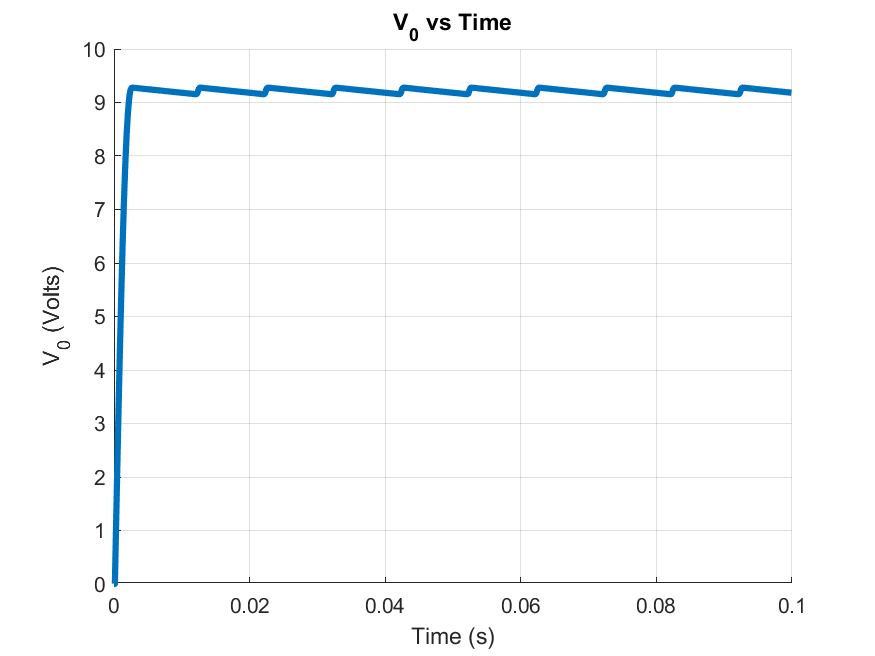
\includegraphics[width = 0.75\textwidth]{5.png}
\caption{Circuit schematic for the step 5}
\end{figure} 

%%%%%%%%%%%%%%%%%%%%%%   EXAMPLE IMAGE FROM PDF   %%%%%%%%%%%%%%%%%%%%%%%%%%%%%%%%
\begin{figure}[H] \centering{
	\includegraphics[scale=0.25]{2a_plot.pdf}}
	\caption{Experiment 2}
\end{figure}
%%%%%%%%%%%%%%%% Deneme Push